%TC:envir minted 1 xall 
%TC:envir algorithmic 1 xall

% Include tables in word count
%TC:envir table 0 word
%TC:envir tabular 1 word

% Include footnotes in word count
%TC:macro \footnote [text]
%TC:macro \footnotetext [text]

%TC:group minted 0 0
%TC:macro \mintinline [ignore]
%TC:macro \colb [ignore]
%TC:macro \hyperref [ignore]


\label{sec:4}

In order to evaluate my project, I take three different approaches, each of which aims to answer one of the questions outlined in \cref{sec:1.1}. \cref{sec:4.1} examines the correctness of my two router prototypes, \cref{sec:4.2} establishes adherence to the official Internet Engineering Task Force's (IETF's) network node standards, and \cref{sec:4.3} compares the performances of the IPv4-only, my IPv6-only, and my dualstack router prototype.



\section{Correctness Evaluation}
\label{sec:4.1}

In \cref{sec:3} I outlined the expected behaviour of each router functionality. These designs were based on packet exchanges with my home router and thus this section takes a test-driven approach to showing router correctness. I use the open-source packet analyser Wireshark to observe the packet exchanges between the hosts and my router prototypes \cite{Wireshark}. I use known network traffic to analyse both my IPv6 and my dual-stack routers.



\subsection{IPv6 Router}
\label{sec:4.1.1}

Both hosts start with initially empty IPv6 neighbour tables. When Host 1 sends an Echo Request to Host 2, it first sends out an NS for Host 2's IPv6 address. The router recognizes the target address and sends back an NA containing the next-hop MAC address. Host 1 places the acquired MAC address in its neighbour table and then goes forward with sending the Echo Request. An exchange of Echo Requests/Replies then begins. \cref{fig:eval-wireshark} shows the packets captured by Wireshark on Host 1's Ethernet port. The router's neighbour entry table is prepopulated and it does not send out NSs of its own. The \texttt{ping} command runs successfully both from Host 1 to Host 2, and the other way around. This exchange shows that the router is parsing and forwarding the packets correctly.

\begin{figure}[htbp]
  \centering
    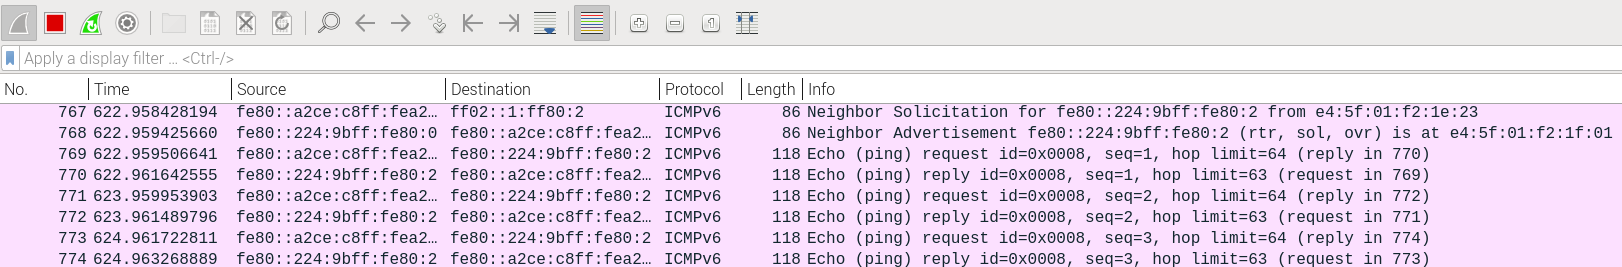
\includegraphics[width=1\textwidth]{figures/evaluation/wireshark.png}
     \caption{Packets captured by Wireshark \cite{Wireshark}. The first two packets (767-768) show \\ an NS/NA exchange with the router. The following packets (769-774) show an exchange \\ of three Echo Requests/Replies between the two hosts.}
     \label{fig:eval-wireshark}
\end{figure}

If either host sends an Echo Request to the router, a similar procedure will occur. The corresponding router subnet's MAC address will be resolved using NDP, and an exchange of Echo Requests/Replies will commence. Each Echo Request is correctly associated with its corresponding Echo Reply and no packet loss occurs. Each Echo Reply comes from the router address that is within the host’s subnet.

These two simple exchanges show that the following router functionalities are working correctly:
\begin{itemize}[topsep=0pt]
\item IPv6 packet parsing (as designed in \cref{sec:3.4.2});
\item IPv6 packet forwarding to a different host (as designed in \cref{sec:3.4.2});
\item ICMPv6 Echo Reply is generated in response to an Echo Request for a router address (as designed in \cref{sec:3.5.2});
\item NDP NA is generated in response to an NS (as designed in \cref{sec:3.6.2}).
\end{itemize}

Two more ICMPv6 functionalities need to be tested, namely the error messages: Time Exceeded and Destination Unreachable. An example test is shown in \cref{fig:eval-timeextest}, where an Echo Request is sent with a Hop Limit of 1. Regardless of what the destination of the Echo Request is, the Time Exceeded error message has the router as its source address, since that is the node at which the Hop Limit expired.
 
\begin{figure}[htbp]
  \centering
    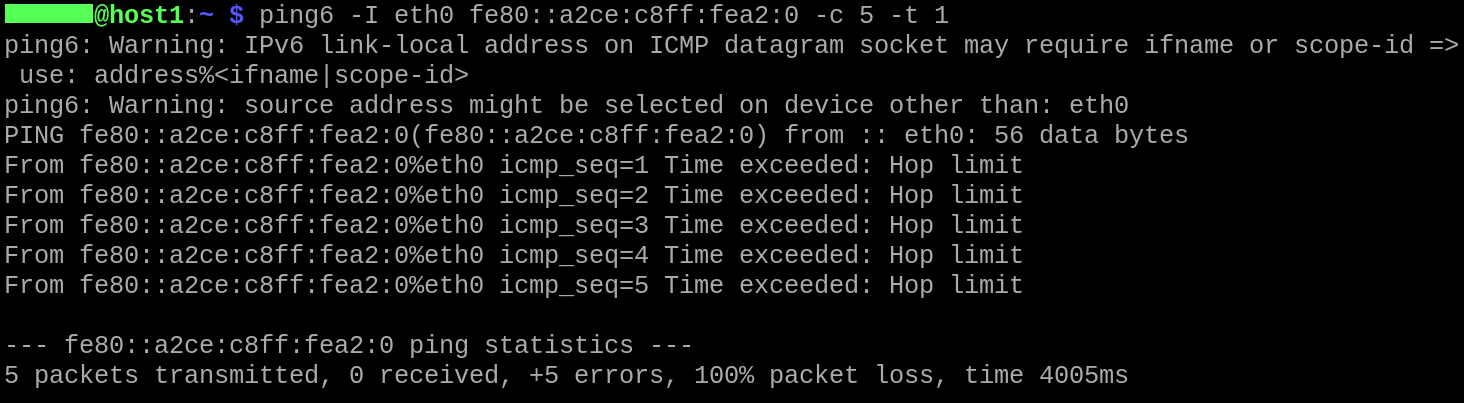
\includegraphics[width=1\textwidth]{figures/evaluation/icmpv6_test2.png}
     \caption{ICMPv6 Time Exceeded error message test.}
     \label{fig:eval-timeextest}
\end{figure}

The Destination Unreachable address requires an extra step to test. If I attempt to ping a random address, I get a Destination Unreachable Code 3 (Address Unreachable) error message from the host itself. This is because the host will send out an NS for this address, but will receive no NA from the router. To get around this, I have to manually define a neighbour table entry for the chosen IPv6 address. Running the \texttt{ping} command then directly sends the Echo Request. The router receives it, and checks its forwarding table to try and find a match for the IPv6 address. When it fails, it sends back a Destination Unreachable Code 0 (No Route to Destination) error message.

It is important to note that depending on which host is conducting these tests, it receives responses from the router address corresponding to the host's subnet. 

These two experiments show that the rest of the router functionalities are performed correctly (all of which were described in \cref{sec:3.5.2}):
\begin{itemize}[topsep=0pt]
\item ICMPv6 Time Exceeded message is generated in response to a Hop Limit expiring;
\item ICMPv6 Destination Unreachable (No Route to Destination) message is generated in response to a miss in the IPv6 forwarding table;
\item Error messages sent back to hosts are sent out the correct router subnet port.
\end{itemize}



\subsection{Dual-Stack Router}
\label{sec:4.1.2}

I run the same tests to establish the correctness of the IPv6 part of the dual-stack router. Similar tests are conducted to verify the IPv4 implementation: ARP Request/Reply, IPv4 forwarding and parsing, ICMPv4 Echo Request/Reply. The P4Pi repository has no ICMPv4 error message functionalities, so those are not tested. Only the IPv6 half of the dual-stack router implements Time Exceeded and Destination Unreachable error messages.

When using the dual-stack router, hosts in the network can send both IPv4 and IPv6 packets to each other, as well as to the router. They can find the next-hop MAC addresses of other devices in the network through either ARP or NDP, and ping both IP router addresses in their respective subnets. The test example below shows that a \texttt{ping} command from Host 1 to Host 2 is successful in eliciting a response in both IPs.

\begin{figure}[htbp]
  \centering
    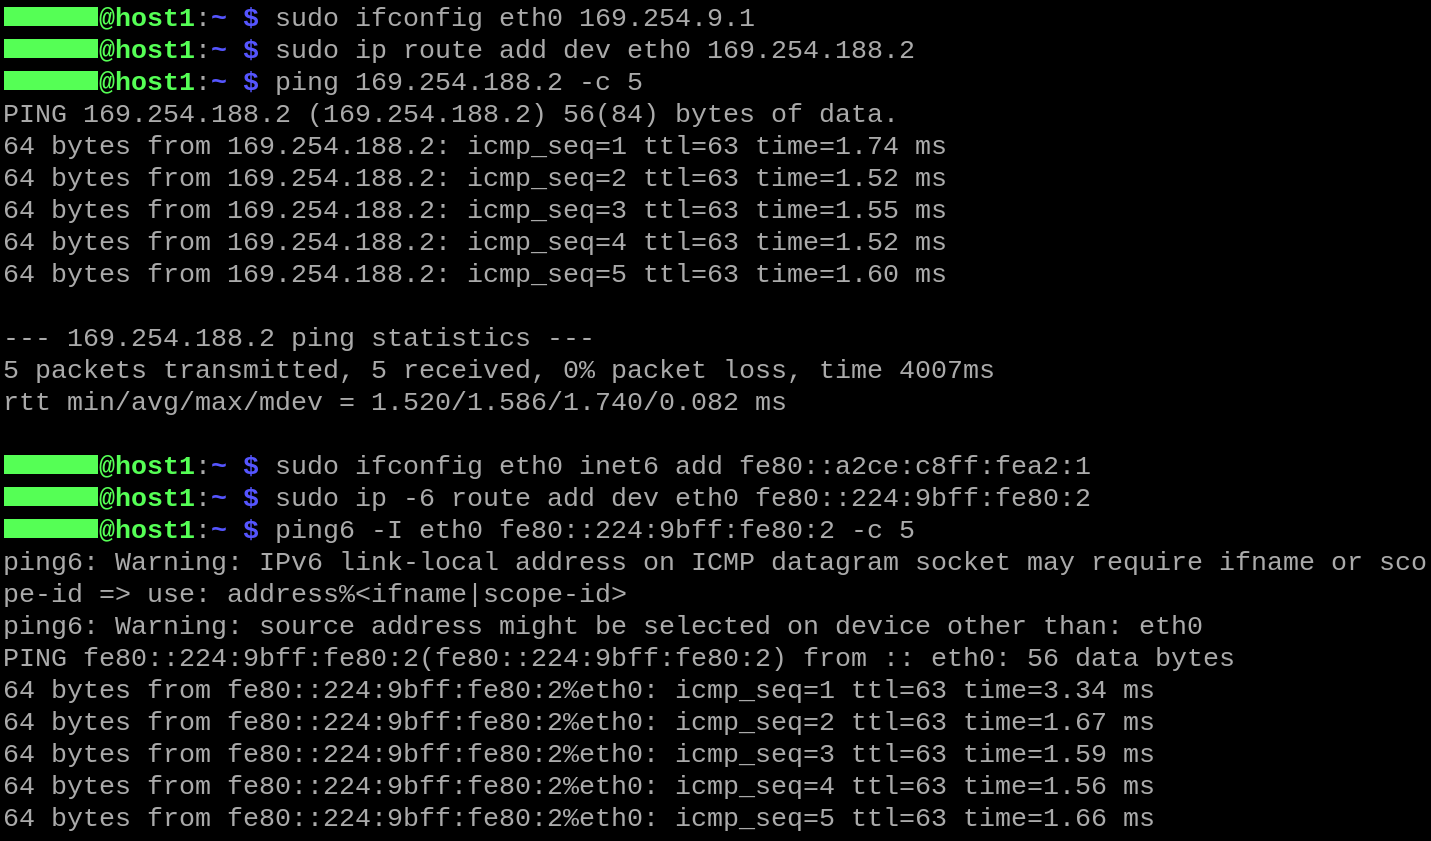
\includegraphics[width=1\textwidth]{figures/evaluation/dualstack_test.png}
     \caption{Dual-stack router successfully forwards both IPv4 and IPv6 packets.}
     \label{fig:eval-dualtest}
\end{figure}



\subsection{Correctness Summary}
\label{sec:4.1.}

This section evaluated and demonstrated the correctness of my router prototype, using the expectations I outlined when building each functionality as a baseline. I test each component and show that it adheres to my individual functionality designs. My final IPv6 router properly parses, forwards and responds to IPv6 packets. It identifies and generates both ICMPv6 and NDP messages. The dual-stack router properly differentiates between IPv4 and IPv6 packets and processes them accordingly. 

By observing the behaviour of both router prototypes through packets captured by Wireshark, I also confirm that checksums are calculated correctly, no packet duplication occurs, and hosts only receive packets which are meant to be received by them.



\section{Standards Compliance Evaluation}
\label{sec:4.2}

In order to functionally evaluate my project, I use the official specifications provided by the IETF Request for Comments (RFC) documentations on IPv6, ICMPv6, NDP, and Dual IP Layering \cite{IPv6Specs, ICMPv6Specs, NDPSpecs, DualStackSpecs}. I compare my router's behaviour with the provided baselines to establish the functional correctness of my project. In \cref{sec:4.2.1} I explain why I chose to use the IETF RFCs as guidelines. In \cref{sec:4.2.2} I provide a general overview of the handling of IPv6 and ICMPv6 packets, as well as the implemented dual-stack functionalities, followed by an in-depth look at specific ICMPv6 message specifications and whether they have been fulfilled in \cref{sec:4.2.3}.



\subsection{What are the IETF RFCs?}
\label{sec:4.2.1}

The Internet Engineering Task Force (IETF) is `the premier standards development organization (SDO) for the Internet', and the Requests For Comments (RFCs) are the IETF's technical documentations \cite{IETFIntro}. The standards produced by the IETF are not obligatory, but are considered best practice by the networking community, and are often adopted by Internet users \cite{IETFIntro}.



\subsection{General Functionalities}
\label{sec:4.2.2}

The following three tables explore the basic router characteristics that I have extracted from the respective specifications. Most of them are intuitive, such as adhering to the defined packet formats or discarding packets that do not fulfil necessary requirements.

\begin{table}[htbp]
    \centering
    \renewcommand{\arraystretch}{1.25}
    \begin{tabular}{|p{125mm}|l|}
    \hline
    \textbf{IETF Specification} & \textbf{Fulfilled?} \\
    \hline
    Supports a link-layer communication facility (Ethernet). & \makecell{\textcolor[RGB]{0,150,0}{\textbf{yes}}} \\
    \hline
    Is consistent with the defined IPv6 header format. & \makecell{\textcolor[RGB]{0,150,0}{\textbf{yes}}} \\
    \hline
    Discards packets that have malformed IPv6 headers. & \makecell{\textcolor[RGB]{0,150,0}{\textbf{yes}}} \\
    \hline
    Supports IPv6 extension header formats. & \makecell{\textcolor[RGB]{200,0,0}{\textbf{no}}} \\
    \hline
    Does not perform checksum verifications or calculations. & \makecell{\textcolor[RGB]{0,150,0}{\textbf{yes}}} \\
    \hline
    Parses, responds to, and forwards packets based on their type, destination address, and data plane forwarding table. & \makecell{\textcolor[RGB]{0,150,0}{\textbf{yes}}} \\
    \hline
    Discards a packet if the Hop Limit is 0 or gets decremented to 0. & \makecell{\textcolor[RGB]{0,150,0}{\textbf{yes}}} \\
    \hline
    Does not support fragmentation. & \makecell{\textcolor[RGB]{0,150,0}{\textbf{yes}}} \\
    \hline
    \end{tabular}
    \caption{IPv6 general specifications \cite{IPv6Specs}.}
    \label{table:eval-ipv6gen}
\end{table}

\begin{table}[htbp]
    \centering
    \renewcommand{\arraystretch}{1.25}
    \begin{tabular}{|p{125mm}|l|}
    \hline
    \textbf{IETF Specification} & \textbf{Fulfilled?} \\
    \hline
    Is consistent with the defined ICMPv6 header format. & \makecell{\textcolor[RGB]{0,150,0}{\textbf{yes}}} \\
    \hline
    Discards packets that have malformed ICMPv6 headers. & \makecell{\textcolor[RGB]{0,150,0}{\textbf{yes}}} \\
    \hline
    Verifies and calculates checksums using an IPv6 pseudoheader. & \makecell{\textcolor[RGB]{0,150,0}{\textbf{yes}}} \\
    \hline
    Uses type codes 0-127 for informational messages. & \makecell{\textcolor[RGB]{0,150,0}{\textbf{yes}}} \\
    \hline
    Uses type codes 128-255 for error messages. & \makecell{\textcolor[RGB]{0,150,0}{\textbf{yes}}} \\
    \hline
    Supports a multitude of ICMPv6 message packets. & \makecell{\textcolor[RGB]{0,150,0}{\textbf{yes}}} \\
    \hline
    \end{tabular}
    \caption{ICMPv6 general specifications \cite{ICMPv6Specs}.}
    \label{table:eval-icmpmv6gen}
\end{table}

\begin{table}[htbp]
    \centering
    \renewcommand{\arraystretch}{1.25}
    \begin{tabular}{|p{125mm}|l|}
    \hline
    \textbf{IETF Specification} & \textbf{Fulfilled?} \\
    \hline
    Has the ability to send and receive both IPv4 and IPv6 packets. & \makecell{\textcolor[RGB]{0,150,0}{\textbf{yes}}} \\
    \hline
    Provides independent correct implementations of an IPv4 node and an IPv6 node. & \makecell{\textcolor[RGB]{0,150,0}{\textbf{yes}}} \\
    \hline
    Provides a configuration switch to disable either the IPv4 or IPv6
    stack (optional). & \makecell{\textcolor[RGB]{200,0,0}{\textbf{no}}} \\
    \hline
    \end{tabular}
    \caption{Dual-stack general specifications \cite{DualStackSpecs}}
    \label{table:eval-dualstackgen}
\end{table}

All basic IPv6 functionalities have been fulfilled, with the exception of extension header formats, as seen in \cref{table:eval-ipv6gen}. The last requirement in the ICMPv6 specifications, \cref{table:eval-icmpmv6gen}, has been marked as `yes' because multiple different ICMPv6 messages have been implemented and the framework for implementing additional messages has been established. This is discussed further in the next section. The dual-stack specifications requirements can be seen in \cref{table:eval-dualstackgen}



\subsection{Specific Message Functionalities}
\label{sec:4.2.3}

The official ICMPv6 specifications define six types of ICMPv6 message: two informational messages (Echo Request and Echo Reply), and four error messages (Destination Unreachable, Packet Too Big, Time Exceeded, and Parameter Problem). As previously described, my IPv6 router implements four of these message types and discards all other ICMPv6 packet types. A breakdown of the required functionalities for these four messages can be seen in the respective tables (\cref{table:eval-destunr}, \cref{table:eval-timeexc}, \cref{table:eval-echo}). All requirements are fulfilled with the exception of an Echo Response to a multicast destination address. My router only responds to unicast Echo Requests. 

The official IPv6 NDP specifications define the expected NDP functionalities of a router. My router responds to NSs with NAs, but its own neighbour entry tables are prepopulated by the control plane, rather than by using NSs. The breakdown of the IETF's requirements for this message pair can be seen in \cref{table:eval-ndpnei}.

In all tables, I use the keywords `MUST' and `SHOULD', as defined by the IETF \cite{KeyWordsSpecs}.

\begin{table}[htbp]
    \centering
    \renewcommand{\arraystretch}{1.25}
    \begin{tabular}{|p{125mm}|l|}
    \hline
    \textbf{IETF Specification} & \textbf{Fulfilled?} \\
    \hline
    A Destination Unreachable message SHOULD be generated by a router in response to a packet that cannot be delivered to its destination address for reasons other than congestion. & \makecell{\textcolor[RGB]{0,150,0}{\textbf{yes}}} \\
    \hline
    If the reason for the failure to deliver is lack of a matching entry in the forwarding node's routing table, the Code field MUST be set to 0. & \makecell{\textcolor[RGB]{0,150,0}{\textbf{yes}}} \\
    \hline
    \end{tabular}
    \caption{ICMPv6 Destination Unreachable specifications \cite{ICMPv6Specs}.}
    \label{table:eval-destunr}
\end{table}

\begin{table}[htbp]
    \centering
    \renewcommand{\arraystretch}{1.25}
    \begin{tabular}{|p{125mm}|l|}
    \hline
    \textbf{IETF Specification} & \textbf{Fulfilled?} \\
    \hline
    If a router receives a packet with a Hop Limit of zero, or if a
    router decrements a packet's Hop Limit to zero, it MUST discard the packet. & \makecell{\textcolor[RGB]{0,150,0}{\textbf{yes}}} \\
    \hline
    The router must also originate an ICMPv6 Time Exceeded message with Code 0 to the source of the packet. & \makecell{\textcolor[RGB]{0,150,0}{\textbf{yes}}} \\
    \hline
    \end{tabular}
    \caption{ICMPv6 Time Exceeded specifications \cite{ICMPv6Specs}.}
    \label{table:eval-timeexc}
\end{table}

\begin{table}[htbp]
    \centering
    \renewcommand{\arraystretch}{1.25}
    \begin{tabular}{|p{125mm}|l|}
    \hline
    \textbf{IETF Specification} & \textbf{Fulfilled?} \\
    \hline
    Every node MUST implement an ICMPv6 Echo responder function that receives Echo Requests and originates corresponding Echo Replies. & \makecell{\textcolor[RGB]{0,150,0}{\textbf{yes}}} \\
    \hline
    The source address of an Echo Reply sent in response to a unicast Echo Request message MUST be the same as the destination address of that Echo Request message. & \makecell{\textcolor[RGB]{0,150,0}{\textbf{yes}}} \\
    \hline
    An Echo Reply SHOULD be sent in response to an Echo Request message sent to an IPv6 multicast or anycast address.  In this case, the source address of the reply MUST be a unicast address belonging to the interface on which the Echo Request message was received.  & \makecell{\textcolor[RGB]{200,0,0}{\textbf{no}}} \\
    \hline
    The data received in the ICMPv6 Echo Request message MUST be returned entirely and unmodified in the ICMPv6 Echo Reply message. & \makecell{\textcolor[RGB]{0,150,0}{\textbf{yes}}} \\
    \hline
    \end{tabular}
    \caption{ICMPv6 Echo Request/Reply specifications \cite{ICMPv6Specs}.}
    \label{table:eval-echo}
\end{table}

\begin{table}[h!tbp]
    \centering
    \renewcommand{\arraystretch}{1.25}
    \begin{tabular}{|p{125mm}|l|}
    \hline
    \textbf{IETF Specification} & \textbf{Fulfilled?} \\
    \hline
    Nodes MUST send Neighbour Advertisements in response to Neighbour Solicitations if they have the target link-layer address in their cache. & \makecell{\textcolor[RGB]{0,150,0}{\textbf{yes}}} \\
    \hline
    The link-layer address for the target option, i.e., the sender of the advertisement, MUST be included on link layers that have addresses when responding to multicast solicitations. & \makecell{\textcolor[RGB]{0,150,0}{\textbf{yes}}} \\
    \hline
    The link-layer address for the target option SHOULD be included when responding to a unicast Neighbour Solicitation. & \makecell{\textcolor[RGB]{0,150,0}{\textbf{yes}}} \\
    \hline 
    A router MUST send out Neighbour Solicitations to acquire link-layer addresses. & \makecell{\textcolor[RGB]{200,0,0}{\textbf{no}}} \\
    \hline 
    \end{tabular}
    \caption{NDP Neighbour Solicitation/Advertisement specifications \cite{NDPSpecs}.}
    \label{table:eval-ndpnei}
\end{table}



\subsection{Standards Compliance Summary}
\label{sec:4.2.4}

This section evaluated whether my routers adhere to the Internet's established best practices, as outlined by the IETF. My router prototypes fulfil all mandatory characteristics of the developed functionalities. Furthermore, my prototypes can easily be extended to implement any additional components, as the core requirements for each protocol have already been built.



\section{Performance Evaluation}
\label{sec:4.3}

In order to compare the performances of the IPv4, IPv6 and dual-stack router prototypes, I simulate network traffic with Echo Request/Reply pairs. I initially sent 100 Echo Request packets from Host 1 to both the router and Host 2, but noticed that the first RTT was always an outlier and, with the help of Wireshark, realised that this is because the hosts' MAC address caches are initially empty. I also noticed unusually high standard deviations, likely caused by the cold cache RTTs. For these reasons, I decided to run two separate experiments: a warm cache experiment and a cold cache experiment. My experiments have limitations, such as each subnet being made up of only one host and the close proximity of the three network nodes. The most important limitation, however, is that I cannot identify the exact points in the network that cause the latency I measure. Different components of every network affect latency differently, often unexpectedly, even when running under identical conditions \cite{LatencyPaper}.



\subsection{Warm Cache Echo Request/Reply}
\label{sec:4.3.1}

The mean warm cache RTTs from 250 Echo Request/Reply pairs are summarized in \cref{table:eval-ping}. The gathered statistics show that the RTTs in both the host-to-host and the host-to-router scenarios are comparable. All four configurations average within the same 150 $\mu$s timespan. \cref{fig:eval-pingWC} shows the cumulative distribution of the warm cache RTTs in a host-to-host exchange and a host-to-router exchange, respectively.

\begin{table}[htbp]
    \centering
    \renewcommand{\arraystretch}{1.25}
    \begin{tabular}{|c|c|c|c|c|}
    \hline
    \multirow{2}{*}{\textbf{IP Protocol}} & \multicolumn{2}{c|}{\textbf{Host-to-Host}} & \multicolumn{2}{c|}{\textbf{Host-to-Router}}\\
    \cline{2-5}
     & \textbf{Single-stack} & \textbf{Dual-stack} & \textbf{Single-stack} & \textbf{Dual-stack}\\
    \hline
    IPv4 & 1.473 $\pm$ 0.128 & 1.531 $\pm$ 0.122 & 0.971 $\pm$ 0.128 & 0.994 $\pm$ 0.108 \\
    IPv6 & 1.544 $\pm$ 0.128 & 1.602 $\pm$ 0.150 & 0.964 $\pm$ 0.094 & 1.004 $\pm$ 0.124 \\
    \hline
    \end{tabular}
    \caption{Mean RTT (ms) from 250 warm cache ping commands with a 95\% confidence \\ interval, obtained by adding and subtracting two standard deviations.}
    \label{table:eval-ping}
\end{table}

\begin{figure}[htbp]
  \centering
    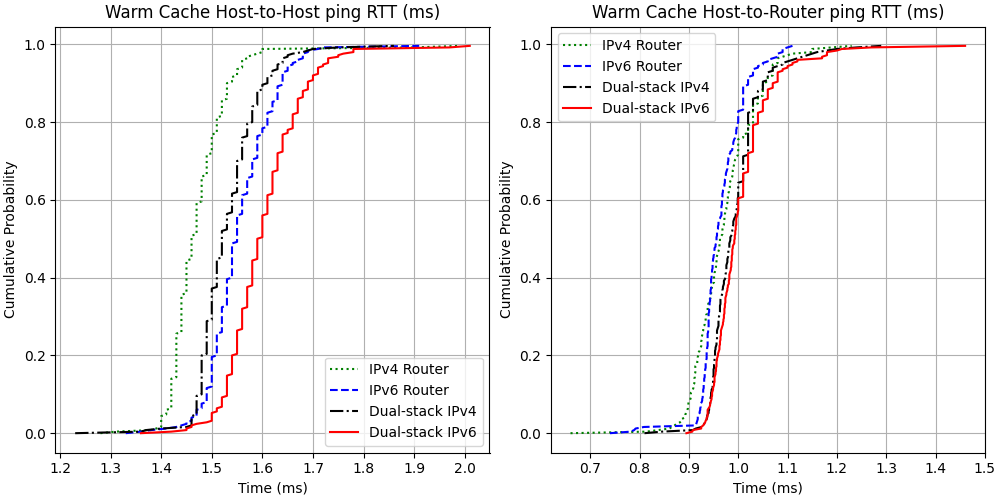
\includegraphics[width=0.90\textwidth]{figures/evaluation/Ping_WC.png}
     \caption{Distributions of warm cache ping RTTs on different configurations when \\ running host-to-host (left) and host-to-router (right).}
     \label{fig:eval-pingWC}
\end{figure}

All distributions exhibit similar slopes and variances. The plots support what could be concluded from \cref{table:eval-ping}. No significant difference is seen between IPv4 and IPv6 in the host-to-router scenario, but the IPv6 mean is 71 $\mu$s higher than the IPv4 mean in the host-to-host scenario. The dual-stack prototype, on average, is 45 $\mu$s slower than the respective single-stack RTTs. There are many reasons for this, such as additional parsing and processing checks, a larger data plane configuration, or simply noise. In both cases, the difference in RTT means falls within the confidence intervals, so no definitive conclusions can be drawn.



\subsection{Cold Cache Echo Request/Reply}
\label{sec:4.3.2}

When running the \texttt{ping} command, the RTT of the first Echo Request/Reply pair is always significantly larger than the rest. This is because Address Resolution/Neighbour Discovery is performed to acquire the next-hop MAC address of the IP address the host is attempting to reach. This information allows us to compare the performances of ARP and NDP. \cref{table:eval-pingCC} shows the RTTs of the first pings after MAC address caches are cleared, and \cref{fig:eval-pingCC} illustrates the collected cold cache data samples as cumulative distribution functions.

\begin{table}[htbp]
    \centering
    \renewcommand{\arraystretch}{1.25}
    \begin{tabular}{|c|c|c|c|c|}
    \hline
    \multirow{2}{*}{\textbf{IP Protocol}} & \multicolumn{2}{c|}{\textbf{Host-to-Host}} & \multicolumn{2}{c|}{\textbf{Host-to-Router}}\\
    \cline{2-5}
     & \textbf{Single-stack} & \textbf{Dual-stack} & \textbf{Single-stack} & \textbf{Dual-stack}\\
    \hline
    IPv4 & 2.770 $\pm$ 0.202 & 2.864 $\pm$ 0.280 & 1.596 $\pm$ 0.244 & 1.748 $\pm$ 0.320 \\
    IPv6 & 3.235 $\pm$ 0.190 & 3.262 $\pm$ 0.240 & 1.746 $\pm$ 0.146 & 1.817 $\pm$ 0.152 \\
    \hline
    \end{tabular}
    \caption{Mean RTT (ms) from 25 cold cache ping commands with a 95\% confidence interval, obtained by adding and subtracting two standard deviations.}
    \label{table:eval-pingCC}
\end{table}

\begin{figure}[htbp]
  \centering
    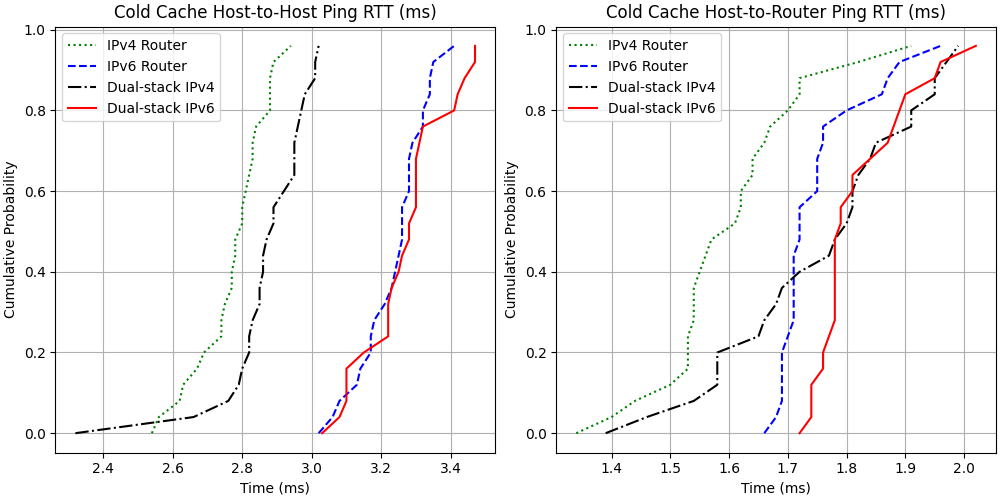
\includegraphics[width=0.90\textwidth]{figures/evaluation/Ping_CC.png}
     \caption{Distributions of cold cache ping RTTs on different configurations when \\ running host-to-host (left) and host-to-router (right).}
     \label{fig:eval-pingCC}
\end{figure}

Observe that IPv6 resolution takes slightly longer than IPv4 resolution. The reason for this is that NDP is part of ICMPv6 and works on top of IPv6, whereas ARP works below IPv4. When developing IPv6, it was decided to integrate NDP into ICMPv6 for efficiency and security reasons which are outside the scope of my dissertation. For the purposes of the gathered results, this means that resolving an NS requires parsing an extra layer of headers, thus takes a margin of time longer than resolving an ARP Request.


\subsection{Performance Summary}
\label{sec:4.3.3}

This section explored the performance of the different router prototypes when simulating identical-purpose traffic in the network. The gathered data shows that the performance of the routers remain stable and suggests that the dual-stack router prototype might be slightly slower than the single-stack routers. NDP is less efficient than ARP, but that is to be expected due to the extra layer of header parsing. Because NDP offers more functionalities than ARP and is only performed once, to establish a connection, the trade-off in efficiency is warranted.

Since any differences in efficiency in the warm cache scenario fall within the confidence intervals, no significant difference in performance can be concluded. Furthermore, the dual-stack router being able to support both IPs greatly benefits networks and outweighs the harm caused by the potentially less efficient packet processing. I thus propose that my router prototypes, both the IPv6 and dual-stack ones, can be used in place of the IPv4 prototype to provide better functionality in a network at a negligible performance cost.



\section{Evaluation Summary}

The evaluation of my project explored correctness, standards compliance and performance. I established that my router prototypes uphold my baseline designs using implementation-driven testing. All design choices were based on observed packet behaviours in working networks. I then compared my router prototypes to the IETF's official specifications and concluded that, for the functionalities that my routers do implement, my routers adhere to the best practices as outlined by the IETF. Finally, I conducted a performance evaluation by running known test traffic in both IPs on both router types (single- and dual-stacked) to establish that there is no significant difference in performance, hence my prototypes can be used in place of the IPv4 prototype to provide better functionality.